%%%% Better Poster latex template example v1.0 (2019/04/04)
%%%% GNU General Public License v3.0
%%%% Rafael Bailo
%%%% https://github.com/rafaelbailo/betterposter-latex-template
%%%% 
%%%% Original design from Mike Morrison
%%%% https://twitter.com/mikemorrison

\documentclass[a0paper,fleqn]{betterposter}
\usepackage{pythonhighlight}
\lstset{
language = Python,
backgroundcolor={\color[gray]{.95}},
breaklines = true,
basicstyle=\fontsize{30}{32}\selectfont\ttfamily,
commentstyle = {\itshape \color[cmyk]{1,0.4,1,0}},
keywordstyle = {\bfseries \color[cmyk]{0,1,0,0}},
stringstyle = {\ttfamily \color[rgb]{1,0,0}},
}

%%%% Uncomment the following commands to customise the format

%% Setting the width of columns
% Left column
%\setlength{\leftbarwidth}{0.25\paperwidth}
% Right column
%\setlength{\rightbarwidth}{0.25\paperwidth}

%% Setting the column margins
% Horizontal margin
%\setlength{\columnmarginvertical}{0.05\paperheight}
% Vertical margin
%\setlength{\columnmarginhorizontal}{0.05\paperheight}
% Horizontal margin for the main column
%\setlength{\maincolumnmarginvertical}{0.15\paperheight}
% Vertical margin for the main column
%\setlength{\maincolumnmarginhorizontal}{0.15\paperheight}

%% Changing font sizes
% Text font
%\renewcommand{\fontsizestandard}{\fontsize{28}{35} \selectfont}
% Main column font
%\renewcommand{\fontsizemain}{\fontsize{28}{35} \selectfont}
% Title font
%\renewcommand{\fontsizetitle}{\fontsize{28}{35} \selectfont}
% Author font
%\renewcommand{\fontsizeauthor}{\fontsize{28}{35} \selectfont}
% Section font
%\renewcommand{\fontsizesection}{\fontsize{28}{35} \selectfont}

%% Changing font sizes for a specific text segment
% Place the text inside brackets:
% {\fontsize{28}{35} \selectfont Your text goes here}

%% Changing colours
% Background of side columns
%\renewcommand{\columnbackgroundcolor}{black}
% Font of side columns
%\renewcommand{\columnfontcolor}{gray}
% Background of main column
%\renewcommand{\maincolumnbackgroundcolor}{empirical}
%\renewcommand{\maincolumnbackgroundcolor}{theory}
%\renewcommand{\maincolumnbackgroundcolor}{methods}
%\renewcommand{\maincolumnbackgroundcolor}{intervention}
% Font of main column
%\renewcommand{\maincolumnfontcolor}{gray}

\begin{document}	
\betterposter{
%%%%%%%% MAIN COLUMN

\maincolumn{
%%%% Main space

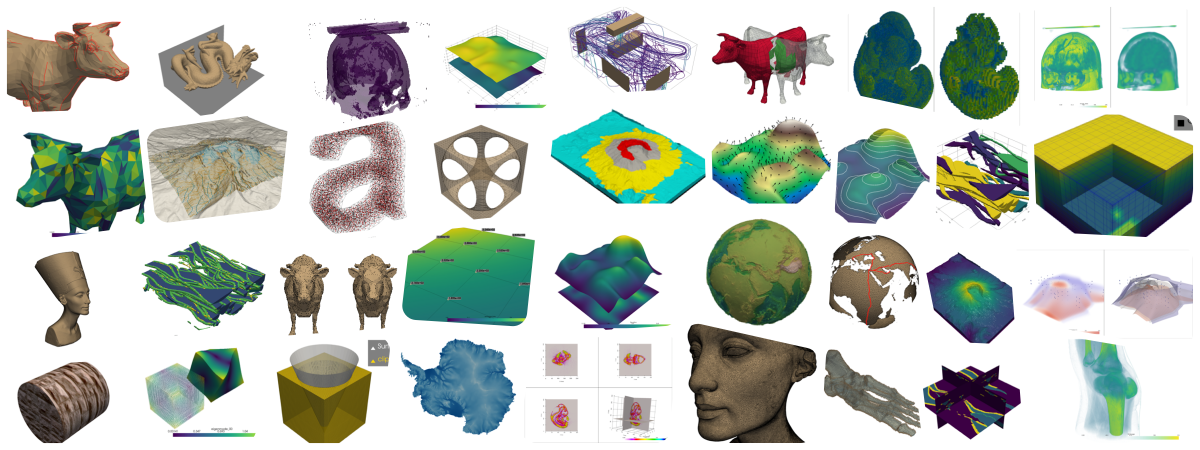
\includegraphics[width=\textwidth]{img/pyvista_banner_small}
\\ Let's plot 3D \textbf{Pythonic} visualization
\\ \$ pip install pyvista
}{
%%%% Bottom space

%% QR code
\qrcode{img/qrcode}{img/smartphoneWhite}{
\textbf{Take a picture} to
\\start tutorial
}
% Smartphone icon
% Author: Freepik
% Retrieved from: https://www.flaticon.com/free-icon/smartphone_65680

%% Compact QR code (comment the previous command and uncomment this one to switch)
%\compactqrcode{img/qrcode}{
%\textbf{Take a picture} to
%\\download the full paper
%}

}

}{
%%%%%%%% LEFT COLUMN


\includegraphics[width=\textwidth]{img/logo}\\

\lstinputlisting[firstline=1, lastline=7]{hello-world.py}

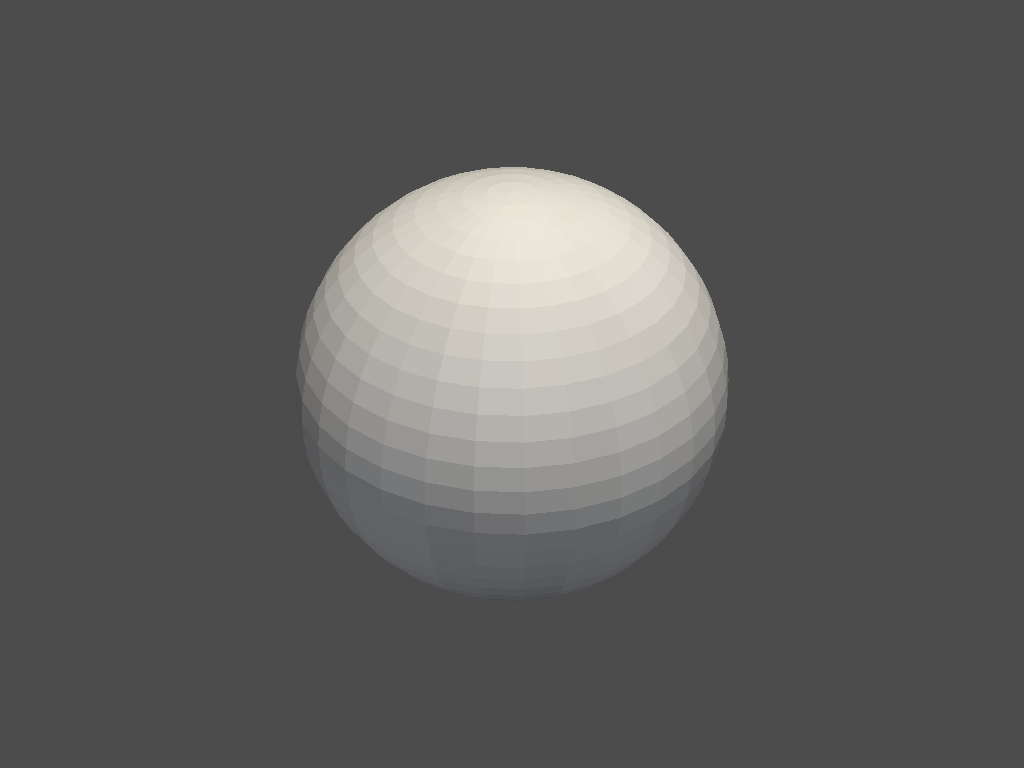
\includegraphics[width=\textwidth]{img/hello-world}

\lstinputlisting[firstline=42, lastline=48]{hello-world.py}

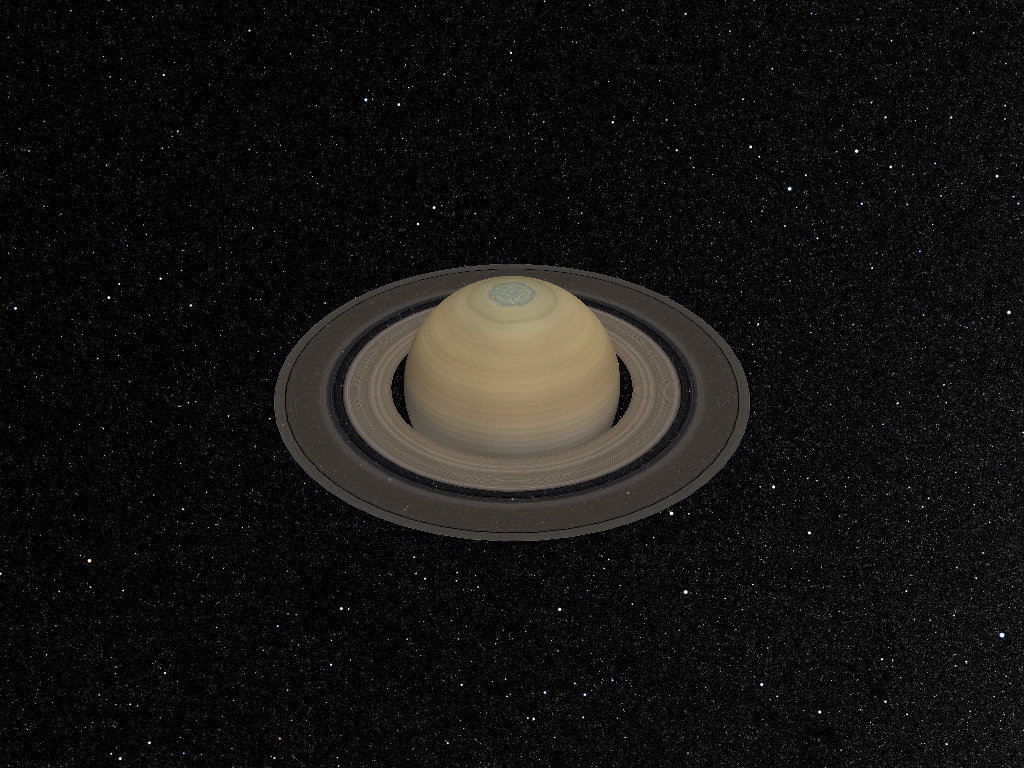
\includegraphics[width=\textwidth]{img/saturn}

\lstinputlisting[firstline=59, lastline=66]{hello-world.py}

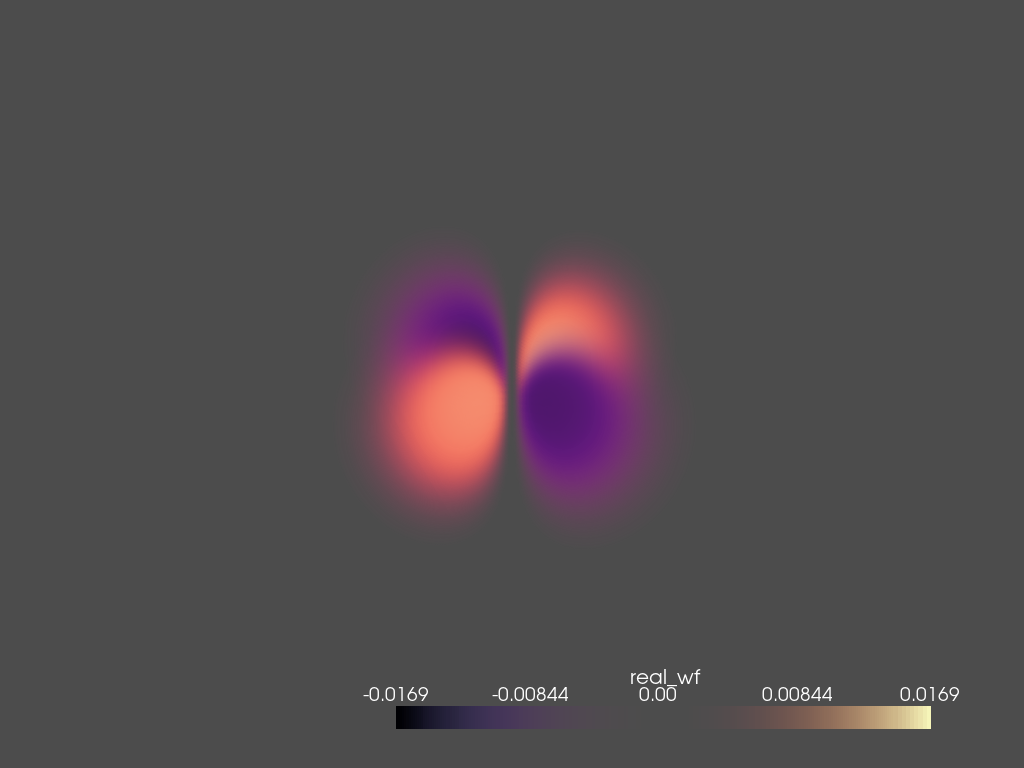
\includegraphics[width=\textwidth]{img/atom}

%% This fills the space between the content and the logo
%% \vfill

}{
%%%%%%%% RIGHT COLUMN

}
\end{document}
